\chapter[SCP-067 艺术家之笔]{
    SCP-067 The Artist's Pen\\
    SCP-067 艺术家之笔
}

\label{chap:SCP-067}

\begin{figure}[H]
    \centering
    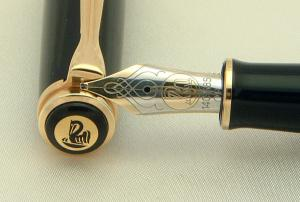
\includegraphics[width=0.5\linewidth]{images/SCP-067.jpg}
    \caption*{SCP-067的笔尖的近照}
\end{figure}

\bb{项目编号:}SCP-067

\bb{项目等级:}Safe

\bb{特殊收容措施:} SCP-067没有用于研究时,保存在一个有毛垫毡的木质盒子中。笔帽需保持盖好,它产生的作品都要提交到SCP研究中心(SCP Research command),用于进一步的研究分析。

\bb{描述:}SCP-067是一支德国产的钢笔(Pelikan),生产时间在一战和二战之间。这支笔是苍绿色的,笔身有一条红线。笔壳是由橡木制作的,笔尖相当锋利,轻轻一按就会扎破皮肤。尽管这支钢笔没有内胆,但是却从来不缺墨水。另外,写出来的墨水种类是(Iron Gall),艺术家常用这种墨水,但是这种墨水很容易腐蚀钢笔。

\begin{figure}[H]
    \centering
    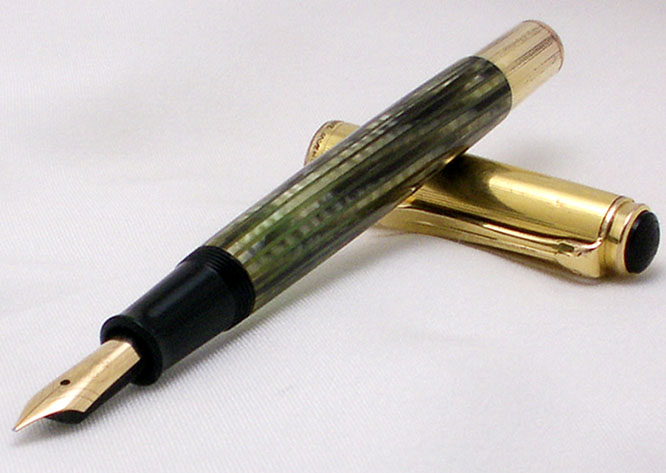
\includegraphics[width=0.5\linewidth]{images/SCP-067-2.jpg}
    \caption*{}
\end{figure}

研究结果推断,所有握住SCP-067的物体会失去手臂的自治权。持有者的知觉没有受损,手臂肘部以下被未知力量控制,理论上是来自SCP-067。其中一种影响是,持笔者在这股力量的控制下开始写作,写下细节详细的自传。自传内容包括持笔者的名字,年龄,生日,犯罪记录,恐惧的东西,等等。有时,持笔者会写生命中的一次事故。例如,当实验对象1204M拿起SCP-067后,他开始描写一年前的一次摩托车事故。后来,实验对象表示他根本想不起来这些细节(实验对象忘记了很多东西,例如之前的车牌号,车的颜色等)。实验对象陈述,当他写作时,感觉当时的事故在脑海中重新发生了一遍,“甚至可以尝到嘴上血的味道”。\\
SCP-067曾经还创作过非常复杂的艺术作品,尽管持笔者完全没有绘画经验。例如,实验对象1102F,一个年轻的女性,没有艺术方面的知识,却画出了一个有翅膀的生物,类似于SCP-███,此例由研究员陈述,现在该研究员身职{[}数据删除]。当实验对象被要求描述当时的感受时,最典型的回答是,他们自愿放弃肢体的控制,以便让SCP-067完成作品(参见引用的回答-01)。尽管实验对象被要求抵抗写作,实验对象却表示有一个意志力强迫他们与SCP-067发生共鸣,钦佩他,赞赏它,并且配合它。

\bb{引用的回答-01:}“我真的不知道该如何解释这一切,它就是发生了。当我拿起笔的一刹那,我的手不再属于我了。我知道我可以移动,但是我不想,我爱那个画出的东西。就好像我的手臂有了生命。后来突然我的手臂停止动作,我又可以控制我的手了,我放下笔。我觉得画出来的东西真是太美了。我猜是笔决定停止的,它在我身上的作用完成了。”

\bb{实验与测试}\\
日期██\slash ██\slash 20██,其它生物使用SCP-067的实验完成。

\bb{实验001:}测试对象,猴子(rhesus macaque),雄性,2岁4个月,已经学会使用笔和记号笔,猴子被放在一间心理监诊室(没有颜色的墙,可单向观察得镜子),房间内有SCP-067,办公桌,一沓纸。

实验对象用左脚捡起SCP-067,然后用右手拿住,接着尝了尝。实验对象把笔放到纸上,开始闻它。30秒之后,实验对象再次拿起笔,用SCP-067敲了敲桌子,又敲了敲自己。实验对象更加用力的敲,直到墨水溅到身上。实验对象惊叫一声将SCP-067丢到地板上(没有受到任何伤害)。

这时,实验对象撕了一张纸,开始擦拭身上的墨水。3分钟之后,实验对象用牙咬住那张纸,从桌子上跳到观察窗的边缘(用的力气把桌子都踢翻了)。实验对象用墨水往观察镜上擦,同时重复发出一些声音;研究分析表明50\%的声音与痛苦有关,另外50\%的声音则意义不明。

实验对象在观察镜上涂抹了6分钟后,用牙齿咬住纸张,然后用手撕扯它,接着丢到地上,此时纸张损毁程度不到20\%。实验对象倒在地板上,开始急促的呼吸,同时发出意义不明的不正常的声音。

驯化者报告说,实验对象从心理监诊室出来后,心情迅速的恢复。在接下来的两个月里,实验对象被紧密监控,但是再也没有发出那种古怪的声音。

有墨水的纸张被存档在{[}数据删除]。
